\chapter{Introduction}

\label{intro} % For referencing the chapter elsewhere, use \ref{intro} 

\section{Problem Description}
With the internet boom of the '90s, many industries have migrated much of their business to the web. Digital commerce is no exception, with Forbes magazine predicting that online sales will continue to grow to a total volume of \$5.8 trillion by 2022. This number would make up over 17\% of all business-to-consumer sales and would be achieved through annual compound growth rates of around 20\% \parencite{forbes2018growth}. The growth in this industry has presented shoppers with an overwhelming number of options to choose from, creating the need for a means for users to filter through the multitude of options \parencite{handbook_1.1_intro}.

The purpose of a  recommender system is to help people make decisions in an area where they do not necessarily have a wealth of personal experience \parencite{rs_1.1_Resnick}. They have been developed to aid users with filtering through wide ranges of options at their disposal to find those offerings most relevant to them. The output of a recommender system is usually in the form of a suggestion to the user, helping them to make decisions such as what items to buy, what music to listen to or what movie to rent \parencite{handbook_1.1_intro}.

As the number of options has grown, so too has the amount of user feedback data. Already in 2007, the online video subscription service Netflix had collected nearly 2 billion ratings from more than 11.7 million subscribers on over 85 thousand titles in its first 10 years of operating. Considering the number of similar streaming and online commerce services, there is indeed an overwhelming number of options for users to choose from -- but also a wealth of data recommender systems can use to make suggestions.
More choices means more feedback, we now have more recorded interactions of what people do -- and \textit{don't} -- like than ever before \parencite{netflix_description}.

Recommender systems can be divided into two categories: \textit{content-based} and \textit{collaborative filtering} models. Collaborative filtering models use only interactions between users and items to learn user preferences, while content-based models make use of meta data such as user demographics or item genres \parencite{handbook_1.5_cf}, \parencite{handbook_1.3_content-based}.

Each of these approaches has its own strengths and weaknesses; however, in both cases the goal when developing a recommender system is typically to predict user preferences. These preferences may be explicit -- e.g. \textit{how will user $u$ rate item $i$?} -- or implicit: \textit{how likely will they be to purchase that item?}

\section{Background to Research}
The Netflix Prize contest in 2008 paved the way for large improvements to the state of the art for predictive ability in collaborative filtering models \parencite{netflix_description}. The contest saw the progression from simpler k-nearest-neighbour models to the use of more advanced latent factor models, achieving a reduction of 10\% in the root mean squared error compared to the previous state of the art \parencite{netflix_bellkor}.

The winning submission to the contest used a matrix factorisation model to achieve state-of-the-art performance in predicting user ratings. This approach used matrix decomposition to factorise the ratings matrix into two smaller matrices, as shown in figure \ref{fig:1_mat-fac} The sizes of these matrices depend on the number of users and items in the dataset \parencite{netflix_bellkor}.

\begin{figure}[H]
\centering
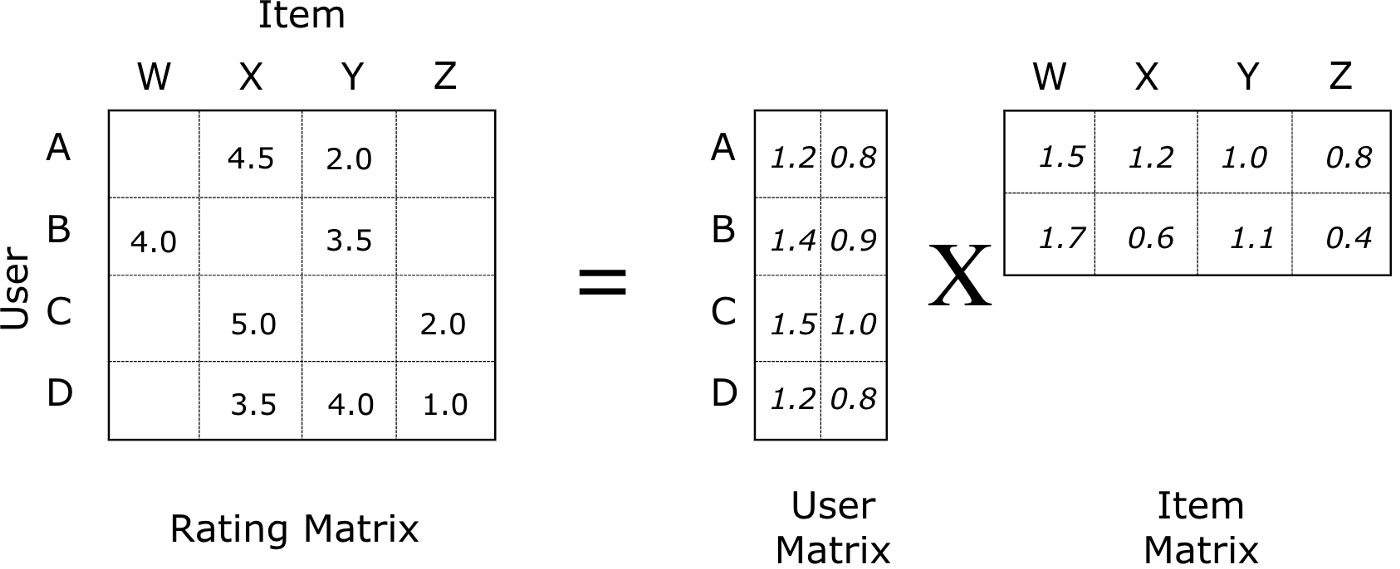
\includegraphics[width=8cm]{Figures/1_matrix-factorisation.png}
\decoRule
\caption[Matrix factorisation]{Matrix factorisation \parencite{liao2018towardsdatascience}}
\label{fig:1_mat-fac}
\end{figure}

The values in each of the two matrices are learned through an alternating least squares method such that the product of the two matrices produces a matrix that is close to the original ratings matrix, but with all missing ratings filled in. Furthermore, it was shown that these latent features are descriptive of the attributes of the items in the dataset and that similar items will have similar latent feature vectors \parencite{koren2009matrix}.

Despite the advances made during the contest, these efforts were untimely as this was before the mainstream adoption of deep learning. Four years after the close of the Netflix Prize contest "AlexNet", utilising the enhanced computational capacity of GPUs for model training, showcased the predictive ability of neural networks with its record-breaking accuracy in the annual ImageNet image classification contest \parencite{krizhevsky2012imagenet}. Since then, the field of deep learning has continued to grow, with neural networks achieving state-of-the-art accuracy on a wide range of problems \parencite{alom2018history}.

\textbf{Come back to this after literature review}   
It has been shown that deep learning can also be applied to collaborative filtering problems. \cite{he2017neural}, used a neural architecture capable of learning the same latent features in users and items as the matrix factorisation methods. The inclusion of hidden layers and non-linear activation functions offered improvements on the previous matrix factorisation methods.

\section{Purpose of the Research}
This minor dissertation explores the potential for using collaborative filtering to predict categorical attributes of items. The aim is not to challenge the state of the art in terms of user rating prediction, but rather to assess the extent to which user-item interactions can be used to predict features such as genres or other common meta data tags which are useful for users when searching through content libraries. The use of latent factors, which have been learned through collaborative filtering, are explored for the purpose of predicting attributes of items.

\section{Layout of the Paper}
The literature review provides an overview of the relevant literature on recommender systems. The chapter covers the methodology surrounding the evaluation of recommender systems and outlines the two main types of models, namely content-based and collaborative filtering models. Particular attention is given to collaborative filtering models applied to explicit feedback data, leading to an in-depth discussion of the models that have been developed to perform this task. These models are visited chronologically, starting with early attempts, then moving onto the notable efforts from the Netflix Prize competition, before outlining some of the more recent approaches using deep learning.

Chapter 3 ...

Chapter 4 ...

Chapter 5 ...

Conclusions and recommendations for further research are outlined in Chapter 6


 